\documentclass[tikz,convert]{standalone}
\usepackage{tikz}
\usetikzlibrary{backgrounds}
\usetikzlibrary{arrows}
\usetikzlibrary{automata}

\usetikzlibrary{snakes}
\tikzset{
  treenode/.style = {align=center, inner sep=0pt, text centered,
    font=\sffamily},
  idle/.style = {treenode, circle, black, font=\sffamily\bfseries, draw=black,
  	text width=1.5em},
  sel_n/.style = {treenode, circle, white, font=\sffamily\bfseries, draw=black,
    fill=black, text width=1.5em},% arbre rouge noir, noeud noir
  opponent_n/.style = {treenode, circle, fill=black, text=white,
     text width=1em, very thick},% arbre rouge noir, nil
  prob_n/.style = {treenode, circle, fill=black,
     text width=1em, very thick},% arbre rouge noir, nil
   prob_reg_n/.style = {treenode, circle, red, draw=red, fill=black,
 	text width=1em, very thick},% arbre rouge noir, nil
    prob_gen_n/.style = {treenode, circle, blue, draw=blue, fill=blue,
 	text width=1em, very thick},% arbre rouge noir, nil
  reg_n/.style = {treenode, circle, red, draw=red, 
    text width=1.5em, very thick},% arbre rouge noir, noeud rouge
  gen_n/.style = {treenode, circle, draw=blue,
    text width=1.5em, very thick},% arbre rouge noir, nil
  sim_n/.style = {treenode, circle, draw=pink,
	text width=1.5em, very thick},% arbre rouge noir, nil
  updated_n/.style = {treenode, circle, draw=green,
  	text width=1.5em, very thick},% arbre rouge noir, nil
  example_n/.style = {treenode, circle, draw=green,
  	text width=2.5em, font=\small, very thick},% arbre rouge noir, nil
}

\newcommand{\prob}[3]{\small $P_{#1}(#2|#3)$}


\begin{document}

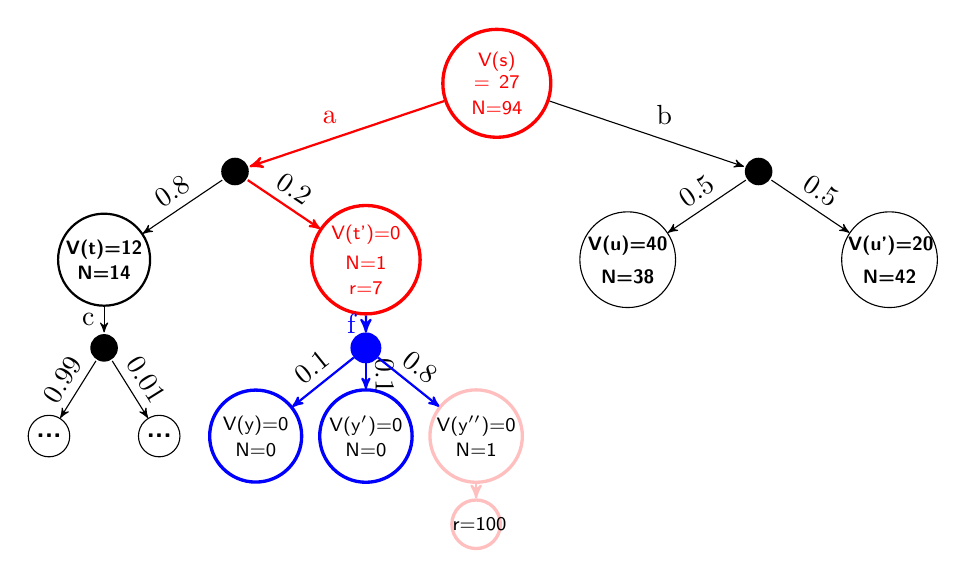
\begin{tikzpicture}[->,>=stealth',level/.style={sibling distance = 9.5cm/#1,
	level distance = 1.6cm},scale=0.7] 

\tikzset{decoration={snake}}
%,post length=0mm,pre length=0mm}}
%\tikzstyle{level 1}=[sibling distance=9cm]
%\tikzstyle{level 2}=[sibling distance=4cm]
\tikzstyle{level 3}=[sibling distance=3cm]
\tikzstyle{level 4}=[sibling distance=2cm]
\tikzstyle{level 5}=[sibling distance=1.5cm]
\node [reg_n, text width=3.2em] {\scriptsize{V(s) = 27\\[-1mm]N=94}}
child{ node [prob_n] {} 
	child{ node [idle, text width=3em] {\scriptsize{V(t)=12\\[-1mm]N=14}} 
		child{ node [prob_n] {}	
			child{ node [idle] {...} 
				edge from parent node[sloped, anchor=south] {0.99}
			} 
			child{ node [idle] {...}         
				edge from parent [draw,black,thin]  node[sloped, anchor=south] {0.01}
			}
			edge from parent   node[left] {c}
		}
		edge from parent [draw,black,thin]   node[sloped, anchor=south] {0.8}
	}
	child{ node [reg_n, text width=3em] {\scriptsize{V(t')=0\\[1mm]N=1\\[-1mm]r=7}}
		child{ node [prob_gen_n] {}	
			child{ node [gen_n, text width=3em] {\scriptsize{V(y)=0\\[-1mm]N=0}} 
				edge from parent node[sloped, anchor=south] {0.1}
			} 
			child{ node [gen_n, text width=3em] {\scriptsize{V(y$'$)=0\\[-1mm]N=0}} 
				edge from parent node[sloped, anchor=south] {0.1}    
			}
			child{ node [sim_n, text width=3em] {\scriptsize{V(y$''$)=0\\[-1mm]N=1}}
				child{ node [sim_n,text width=1.7em] {\scriptsize{r=100}}
					edge from parent [draw,thick,pink,decorate] node {}
				}     
				edge from parent node[sloped, anchor=south] {0.8}    
			}
			edge from parent [draw,thick,blue] node[left] {f}
		}
		edge from parent node[sloped, anchor=south] {0.2}
	}                            
	edge from parent [draw,red,thick] node[above left] {a} 
}   
child{ node [prob_n] {}
	child{ node [idle, text width=3em] {\scriptsize{V(u)=40\\N=38}} 
%		child{ node [prob_n,xshift=30.0] {}
%			child{ node [idle] {$w$}
%				edge from parent node[sloped, anchor=south] {0.5}
%			}
%			child{ node [idle] {$w'$}
%				edge from parent node[sloped, anchor=south] {0.5}
%			}
%%		}
%		child{ node [prob_n,xshift=30.0] {} 
%			child{ node [idle] {$x$}
%				edge from parent node[sloped, anchor=south] {0.99}
%			}
%			child{ node [idle] {$x'$}
%				edge from parent node[sloped, anchor=south] {0.01}
%			}
%			edge from parent node[above right] {c}
%		}
		edge from parent node[sloped, anchor=south] {0.5}
	} 
	child{ node [idle, text width=3em] {\scriptsize{V(u')=20\\N=42}}         
		edge from parent node[sloped, anchor=south] {0.5}    
	}
	edge from parent node[above right] {b}
}

; 
\end{tikzpicture}
\end{document}
